\documentclass[journal,comsoc]{IEEEtran}

\IEEEoverridecommandlockouts 

\usepackage{amsmath}
%\usepackage{amsthm}
\usepackage{amssymb}
\usepackage[justification=justified,font=footnotesize]{caption}
%\usepackage{cancel}
%\usepackage{enumerate}
%\usepackage[stable]{footmisc}
\usepackage{fancyvrb}
\usepackage{graphicx}
%\usepackage{hyperref}
\usepackage[utf8x]{inputenc}
\usepackage{color,listings}
%\usepackage{mathpartir}
%\usepackage{relsize}
%\usepackage{setspace}
%\usepackage{stmaryrd}
%\usepackage{listings}
%\usepackage{placeins}
\usepackage{multicol}
%\usepackage{txfonts}
\usepackage{url}
\usepackage[all]{xy}
%\usepackage{tikz}
%\usetikzlibrary{arrows,shapes,decorations.pathmorphing,backgrounds,positioning,fit,petri}
\usepackage[T1]{fontenc}% optional T1 font encoding
\usepackage{amsmath}
\usepackage{fancyhdr}
%\usepackage{kantlipsum}
%\interdisplaylinepenalty=2500
%\usepackage[cmintegrals]{newtxmath}
\usepackage{eso-pic}


%\usepackage[titles]{tocloft}
%\renewcommand{\cftchapfont}{\bfseries}
%\usepackage[Conny]{fncychap}
%\ChNameVar{\centering\Large\rm\bfseries}
%\ChNumVar{\Large}
%\ChRuleWidth{1pt}
%\ChTitleVar{\centering\Large\rm}

\usepackage{array}
\usepackage{mdwmath}
\usepackage{mdwtab}
\usepackage{eqparbox}

% predefined names
\newcommand{\pvslm}{\textsf{pvslm}}


\usepackage[T1]{fontenc}% optional T1 font encoding
\usepackage{amsmath}
\usepackage{fancyhdr}
\usepackage{kantlipsum}
\interdisplaylinepenalty=2500
\usepackage[cmintegrals]{newtxmath}

% correct bad hyphenation here
\hyphenation{op-tical net-works semi-conduc-tor}

\fancypagestyle{plain}{
  \fancyhf{}
  \fancyhead[C]{IEEE 11CCC 2016}     %% C or L or R.
  %\fancyfoot[L]{This is a notice}%                        %% C or L or R.
  \renewcommand{\footrulewidth}{0pt} 
  \renewcommand{\headrulewidth}{0pt}
}
\usepackage{eso-pic}

\begin{document}

\AddToShipoutPictureBG*{%
  \AtPageUpperLeft{%
    \setlength\unitlength{1in}%
    \hspace*{\dimexpr0.5\paperwidth\relax}%%  change \dimexpr0.5\paperwidth\relax appropriately
    \makebox(0,-0.75)[c]{\Large IEEE 11CCC 2016}%
}}

\title{Library Management for PVS}

%\author{\authorblockN{Miguel Romero}
%\authorblockA{Escuela Colombiana de Ingenier\'{i}a\\
%Bogot\'{a}, Colombia\\
%Email: miguel.romero@mail.escuelaing.edu.co}
%\and
%\authorblockN{Camilo Rocha}
%\authorblockA{Pontificia Universidad Javeriana \\
%Cali, Colombia\\
%Email: camilo.rocha@javerianacali.edu.co}}

\author{
\IEEEauthorblockN{Miguel Romero\IEEEauthorrefmark{1}, Camilo Rocha\IEEEauthorrefmark{2}\\}
    \IEEEauthorblockA{\IEEEauthorrefmark{1}Escuela Colombiana de Ingenier\'{i}a - Bogot\'{a}, Colombia. Email: miguel.romero@mail.escuelaing.edu.co\\}
    \IEEEauthorblockA{\IEEEauthorrefmark{2}Pontificia Universidad Javeriana - Cali, Colombia. Email: camilo.rocha@javerianacali.edu.co}
}

\maketitle

\begin{abstract}
  The Prototype Verification System (PVS) is a specification language
  integrated with support tools and a theorem prover. One mechanism
  for extending and improving PVS is via the development of libraries,
  i.e., collections of mechanized theories in the language of
  PVS. This paper presents the $\pvslm$ tool: (i) a description
  language for annotating PVS libraries, with a small footprint but
  expressive enough for describing dependencies among library
  theories; and (ii) an implementation for managing PVS libraries
  annotated with this language, offering support for several library
  sources.  The usefulness of the $\pvslm$ tool is illustrated with a
  detailed step-by-step guide on how to manage the latest version of
  the NASA PVS Library, which is currently annotated with $\pvslm$'s
  description language.
\end{abstract}


\begin{IEEEkeywords}
PVS, PVSLM, PVS Library Manager, PVS theory, Git, Python
\end{IEEEkeywords}

% For peerreview papers, this IEEEtran command inserts a page break and
% creates the second title. It will be ignored for other modes.
\IEEEpeerreviewmaketitle

\section{Introduction}
\label{sec.intro}


The Prototype Verification System~\cite{pvs-cade92} (PVS) is a
verification system comprising a specification language integrated
with support tools and a theorem prover; basically, PVS is a
mechanization of classical typed higher-order logic with
specifications organized into parameterized theories in this logic.
The PVS system has been used in state-of-the-art formal methods
projects as a productive environment for constructing and maintaining
collections of theories, both in industry and in research. These novel
developments often result in large collections of PVS definitions,
theorems, and proofs, grouped into libraries, with many dependencies
among them. This is the case, for instance, of the NASA PVS
Library~\cite{nasalib} maintained by the NASA Langley Formal Methods
Team: a large collection of freely-available formal developments in
PVS comprising more than 40 theories, 24000+ theorems, and 136000+ and
3623000+ lines of, respectively, specification and proofs, all of
theses ranging from trigonometry to graphs and topology.  In general,
given the increasing size of mathematical developments in the form of
libraries and the growing need for and adoption of mechanized proof
environments~\cite{avigad-mech14,hales-proofs14} such as PVS, it is
important to have tools for managing such libraries.

This paper presents $\pvslm$~\cite{pvslm}, an utility for assisting in
the management of PVS libraries, comprising: (i) a description
language for annotating PVS libraries, with a small footprint but
expressive enough for describing complex dependencies among library
theories; and (ii) an implementation for managing PVS libraries
annotated with this language, offering support for several library
sources. In $\pvslm$, the description language is designed to
represent a PVS library as a collection of packages, with a package
consisting of a collection of PVS theories. In this sense, the
annotations can help in documenting each library with the information
of the theories it offers and their dependencies, so it can be shared
among PVS users with the help of the $\pvslm$ implementation. The
$\pvslm$ implementation is a command line tool offering support for
adding, updating, deleting, and re-installing the contents of a
library source, and also managing several library sources at the same
time.

The $\pvslm$ description language is presented in this paper with the
help of BNF-like notation. The $\pvslm$ implementation is written in
the Python programming language and it can manage {\em any}
(annotated) PVS library that is publicly available from a $\pvslm$
server through the internet: once available, such a library source can
be configured in $\pvslm$, be automatically downloaded from the
internet, and set up in the host system. As a case study for the use
of the $\pvslm$ tool, this paper presents a step-by-step guide on how
to manually configure the NASA PVS Library comprising the command line
instructions and snapshots of the user interaction.

The current distribution of \verb$pvslm$ is freely available for
download~\cite{pvslm} under the GNU General Public License GPLv3 and
it automatically installs the latest version of the NASA PVS Library,
which is currently annotated with the $\pvslm$ description language.

\paragraph{Paper outline.} Section ~\ref{sec.conf} presents the $\pvslm$ 
description language. Sections ~\ref{sec.install} and ~\ref{sec.cmd} 
present, respectively, instructions for obtaining and installing the $\pvslm$ 
implementation, and a list of commands available from $\pvslm$. 
Section ~\ref{sec.nasalib} includes a step-by-step guide on the configuration and
installation with $\pvslm$ of the NASA PVS Library. Some concluding
remarks are presented in Section ~\ref{sec.concl}.


\section{The $\pvslm$ Description Language}
\label{sec.conf}

This section presents a formal definition of the $\pvslm$ description
language in the form of BNF-like notation. It also presents the main
conventions and assumptions used by the $\pvslm$ tool for managing PVS
libraries.


\paragraph{Terminology.}
The $\pvslm$ tool distinguishes three levels of aggregation for PVS
sources. A PVS theory is the building block of a library managed by
$\pvslm$. A {\em package} is a collection of theories.  A {\em
  library} is at the top level of aggregation, comprising a collection
of packages. In summary, a library is a collection of packages and a
package is a collection of theories. The $\pvslm$ tool can manage
several libraries each with several packages.

\paragraph{Package configuration.}
A package is defined in a folder at the root of the library source,
with the folder name defining the name of the package. Each folder
contains the \cde{pvs} and \cde{prf} files for its theories, and a
folder named \cde{pvsbin}: this is a special folder used by the
$\pvslm$ implementation for accessing the {\em package metadata} from
a file named \cde{top.dep}.

\paragraph{Package metadata.} The metadata of a package is defined
in its \cde{top.dep} file, located inside folder
\cde{pvsbin}. Table~\ref{tab.bnf} presents the syntax of $\pvslm$
description language, in BNF-like notation, used to populate this
metadata file.


\begin{table}
  \centering
  \begin{tabular}{r c p{8cm}}
    \hline \\
    $\nterm{\cde{metadata}}$ & ::= & $\nterm{\cde{header}} \; \nterm{\cde{body}}$ \\
    $\nterm{\cde{header}}$ & ::= & `/' $\nterm{\cde{theorylist}}$ \\
    $\nterm{\cde{theorylist}}$ & ::= & $\nterm{\cde{theory}} \mid \nterm{\cde{theory}}$ `,' $\nterm{\cde{theorylist}}$ \\
    $\nterm{\cde{body}}$ & ::= & $(\nterm{\cde{packagedep}} \mid \nterm{\cde{theorydep}})*$ \\
    $\nterm{\cde{packagedep}}$ & ::= & $\nterm{\cde{package}}$ `/' $\nterm{\cde{theorylist}}$ \\
    $\nterm{\cde{theorydep}}$ & ::= & $\nterm{\cde{theory}}$ `:' $\nterm{\cde{qualtheorylist}} ?$ \\
    $\nterm{\cde{qualtheorylist}}$ & ::= & $\nterm{\cde{qualtheory}} \mid \nterm{\cde{qualtheory}}$ `,' $\nterm{\cde{qualtheorylist}}$ \\
    $\nterm{\cde{qualtheory}}$ & ::= & $(\nterm{\cde{package}}\; \text{`@'})?$ $\nterm{\cde{theory}}$ \\
    \\
    \hline
  \end{tabular}
  \caption{Syntax of the \cde{top.dep} metadata file in NASALib.}
  \label{tab.bnf}
\end{table}

The topmost symbol in the description language is
$\nterm{\cde{metadata}}$, while $\nterm{\cde{theory}}$ and
$\nterm{\cde{package}}$ are terminals representing, respectively,
theory and package names. The metadata comprises two parts, namely, a
header and a body. The header corresponds to a single line with an `/'
symbol followed by a comma-separated list of theory names; these names
correspond to the names of the theories included in the package (in
any order). A body comprises any number of lines, each with either a
package dependency or a theory dependency. A package dependency
describes a dependency from another package and the list of theories
from that package that are being depended upon. A theory dependency
describes, for each one of the theories listed in the header of the
package, the list of its theory dependencies. In the case such a
theory depends on a theory from other package, the name of that
dependency must be qualified by the name of its package.

Figure~\ref{fig.top} presents an overview of the configuration file
for package \cde{trig} in NASALib. According to its header
description, package \cde{trig} defines theories \cde{top},
\cde{trig\_doc}, \cde{trig}, \cde{trig\_values}, etc. It contains $5$
package dependencies and $6$ theory dependencies. For instance,
package \cde{trig} depends on theory \cde{for\_iterate} in package
\cde{structures}, and on theories \cde{finite\_sets\_minmax} and
\cde{finite\_sets\_inductions} in package \cde{finite\_sets}. On the
other hand, theory \cde{trig\_doc} has no dependencies, while theory
\cde{trig} depends on theories \cde{trig\_basic}, \cde{sqrt},
\cde{trig\_values}, and \cde{trig\_ineq}. In the case of theory
\cde{sqrt}, it is explicitly stated that such a theory is in package
\cde{reals}.

\begin{figure}
  \centering
  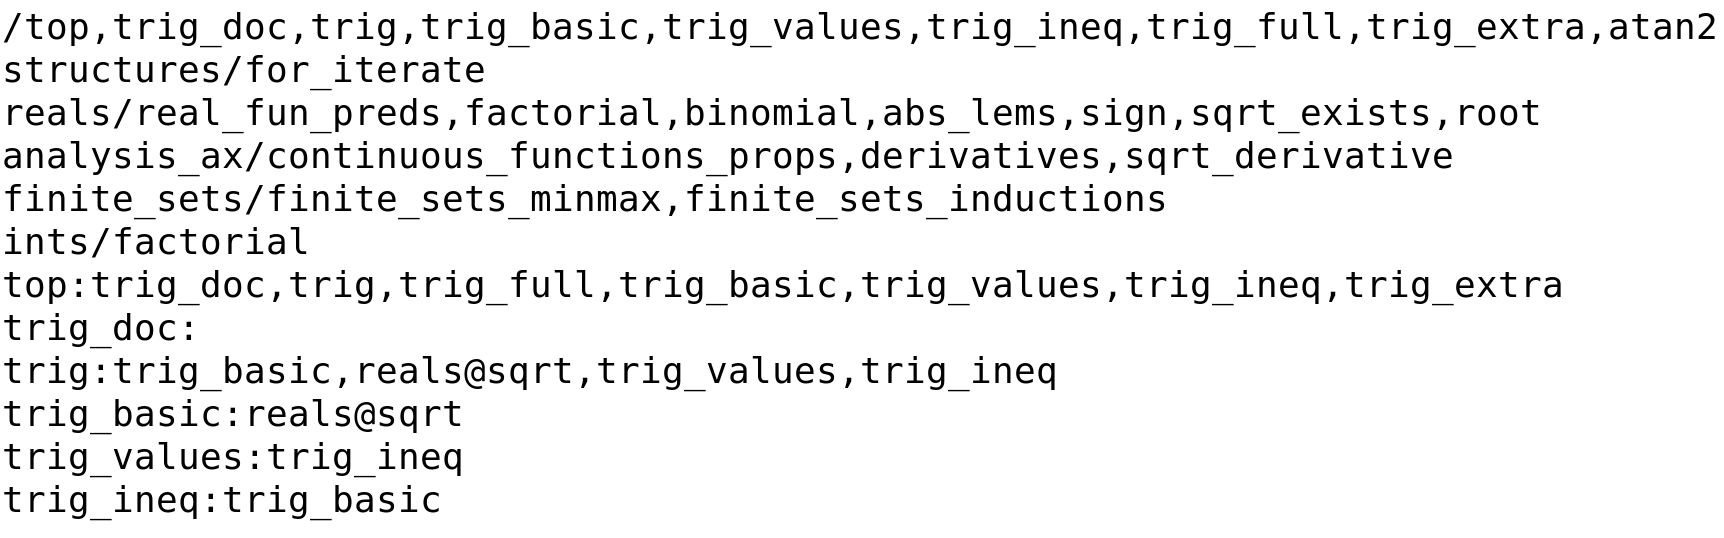
\includegraphics[width=11cm]{images/top.png}
  \caption{Overview of metadata file for package \cde{trig} in NASALib.}
  \label{fig.top}
\end{figure}


\section{Installation and Architecture}
\label{sec.install}

This section presents an overview of the installation procedure and
the distributed architecture of $\pvslm$.

The $\pvslm$ tool can be installed automatically from the command line
by issuing the following command:
%
\begin{verbatim}
  curl http://migueleci.github.io/pvslm/downloads/pvslm-conf.py \
    -o pvslm-install && chmod +x pvslm-install && \
    python ./pvslm-install
\end{verbatim}
%
This command uses the $\curl$ utility to download the $\pvslm$
installation sources from GitHub. Once these sources are downloaded
and some file permissions adjusted, the installation process is
executed as a Python 2 script. During the installation process, the
user can select the location in which the tool is to be installed,
including where the configuration files for the library sources and
the local copy of the libraries are to be placed. This script has been
tested both on Linux and Mac OS X boxes. Figure~\ref{fig.install}
depicts a successful installation procedure of $\pvslm$ in a Ubuntu
Linux box.

\begin{figure}
  \centering
  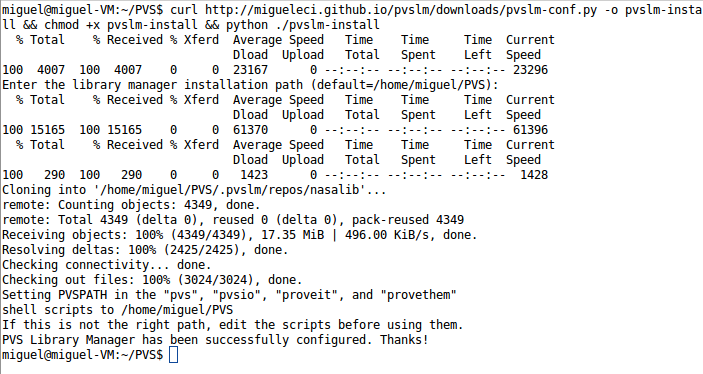
\includegraphics[width=11cm]{images/install.png}
  \caption{A successful installation procedure of $\pvslm$ in a Ubuntu
    Linux box.}
  \label{fig.install}
\end{figure}

Upon its successful installation, $\pvslm$ automatically configures
the NASALib library sources and makes a local copy of them by using
Git's clone command, so they are available for installation in PVS.

The $\pvslm$ tool is desiged with a distributed architecture. It can
connect to library sources over the internet. Each time a source is
configured, $\pvslm$ can download the library into the host system as
a local $\git$ repository. Further updates of the library are carried
out internally by $\pvslm$ by using $\git$'s pull
command. Figure~\ref{fig.arch} depicts the architecture of
$\pvslm$. It is important to note that although GitHub is used as
$\git$ server of reference throughout this paper, it is also possible
to use other publicly available servers such as BitBucket, for
instance, containing an annotated library.

\begin{figure}
  \centering 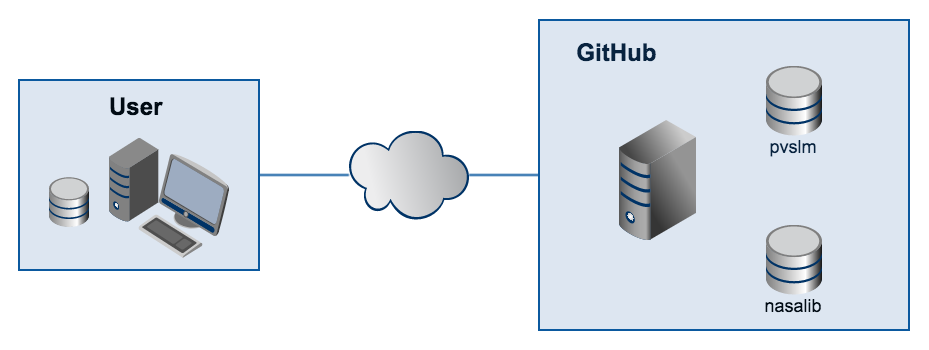
\includegraphics[width=11cm]{images/arch.png}
  \caption{Distributed architecture of $\pvslm$.}
  \label{fig.arch}
\end{figure}


\section{Available Commands}
\label{sec.cmd}

This section presents the list commands offered by the $\pvslm$
tool. Section~\ref{sec.nasalib} presents examples on the use of some
of these commands.

The $\pvslm$ tool provides commands at two levels. First, it provides
commands at the level of library sources for managing library $\git$
repositories.  Second, it provides commands at the level of packages
for managing the contents of a library. Table~\ref{tab.cmd} lists all
commands $\pvslm$ offers.

At the level of library sources, the tool provides $5$ different
commands, all identified with the special token \cde{src}. They
include commands for:

\begin{itemize}
  \item Adding a library source (i.e., command \cde{-a}) with a
    name, a short description, and a $\git$ URL.
  \item Deleting a library source (i.e., command \cde{-d}) with
    the given name.
  \item Cloning a library source (i.e., command \cde{-c}) with the
    given name.
  \item Updating a library source (i.e., command \cde{-u}) with
    the given name.
  \item Removing the clone of a library source (i.e., command
    \cde{-r}) with the given name.
\end{itemize}

It is important to note that none of the commands at the library
source level modify the user's PVS installation. These commands
exclusively modify the internals of the $\pvslm$ configuration. Also,
note that a library source is realized exactly by one $\git$
repository.

At the level of packages, the tool provides $4$ different
commands, all identified with the special token \cde{pkg}. They
include commands for:

\begin{itemize}
  \item Installing and updating a given package (i.e., command
    \cde{-i}) from a given library source, including {\em all} its
    dependencies.
  \item Updating a given package (i.e., command \cde{-u}) from a given
    library source, including {\em all} its dependencies.
  \item Deleting a given package (i.e., command \cde{-d}) from a given
    library source (local copy), including all packages that depend on
    it.
  \item Listing the contents (i.e., command \cde{-l}) from a given
    library source.
\end{itemize}

Note that listing command has three variants. In the first case, all
libraries available to the system are listed. In the second case, all
packages of a given library are listed. In the third case, all
dependencies of a given package and library are listed. Internally,
the $\pvslm$ uses a topological sorting algorithm, based upon each
package's metadata, for computing the set of dependencies among
theories and packages.

\begin{table*}[pthb]
  \begin{center}
    \begin{tabular}{ | l | l | l | p{6cm} | }
      \hline Level & Command & Parameters & Description \\ \hline
      src & -a          & name desc URL         & Add a new library source with the given name, description, and URL.                   \\ \cline{2-4}
          & -d          & name                  & Delete the given library source.                                          \\ \cline{2-4}
          & -c          & name                  & Clone the given library source.                          \\ \cline{2-4}
          & -u          & name                  & Update the given library source.                                \\ \cline{2-4}
          & -r          & name                  & Remove the clone of the given library source.                                                  \\ \hline
      pkg & -i          & library@package       & Install and update the given package, and all its dependencies.                \\ \cline{2-4}
          & -u          & library@package       & Update a package and all its dependencies.                   \\ \cline{2-4}
          & -d          & library@package       & Delete a  package and all ones depending on it.           \\ \cline{2-4}
          & -l          &                       & List the installed libraries.                                       \\ \cline{2-4}
          & -l          & library               & List the available packages of the given library.                         \\ \cline{2-4}
          & -l          & library@package       & List all the dependencies of the given package.                               \\ \hline
    \end{tabular}
  \end{center}
  \caption{$\pvslm$ command list.}
  \label{tab.cmd}
\end{table*}



\section{Case study: Managing NASALib with $\pvslm$}
\label{sec.nasalib}

This section presents a step-by-step guide on the configuration and
installation of the NASA PVS Library (NASALib) with the help of the
$\pvslm$ implementation. The current release of NASALib is annotated
with $\pvslm$'s description language and it is freely available from a
$\git$ repository in GitHub.

\paragraph{Library source creation.}
The first step is to issue a command for configuring the library sources
as follows:
%
{\small\begin{verbatim}
  $ pvslm.py src -a \\
      nasalib \\
      `The NASA PVS Library is a collection of formal PVS developments \\
         maintained by the NASA Langley Formal Methods Team.' \\
      https://github.com/nasa/pvslib.git
\end{verbatim}}
%
\noindent This command generates the library source configuration file
in the $\pvslm$ installation folder with the given information: a
library named \cde{nasalib}, with the given description, and whose
packages are available as a $\git$ repository from the given URL. At
this point, the configuration file is created but no packages are
downloaded nor installed from the repository. Note that it is not
possible to have two or more library sources with the same name.

It is important to note that this step is unnecessary with the current
distribution of $\pvslm$ because its installation script automatically
creates a library source configuration file for \cde{nasalib}. This
step is included for the sake of completeness of the example.

\paragraph{Downloading a library.} It is possible to use the $\pvslm$
implementation for downloading a library once its library source file
has been created. The following command downloads NASALib:
%
{\small\begin{verbatim}
  $ pvslm.py src -c nasalib
\end{verbatim}}
%
Internally, this command uses $\git$'s cloning technology so that the
NASALib repository is copied locally from the URL configured with the
library source.

\paragraph{Updating a library.} It is also possible to update a local
copy of a library. For updating the local copy of NASALib, an user can
issue the following command:
%
{\small\begin{verbatim}
  $ pvslm.py src -u nasalib
\end{verbatim}}
%
The effect of this command is to update the entire local copy of
\cde{nasalib} via $\git$'s pull command from the URL configured with
the library source.

\paragraph{Listing the contents of a library.} Once a local
copy of a library is available, it is possible to list all its
packages and their dependencies. The following command can be issued
to list the dependencies of package \cde{complex} in NASALib:
%
{\small\begin{verbatim}
  $ pvslm.py pkg -l nasalib@complex
\end{verbatim}}
%
The output of this command is as follows:
%
{\small\begin{verbatim}
  Package complex depends on:
  algebra
  analysis_ax
  ints
  lnexp
  reals
  structures
  trig
\end{verbatim}}

\paragraph{Installing a package in PVS.} The $\pvslm$ implementation
can install a package from a local copy of a library in a working PVS
environment. The following command installs package \cde{complex} from
NASALib:
%
{\small\begin{verbatim}
  $ pvslm.py pkg -i nasalib@complex
\end{verbatim}}
%
Since package \cde{complex} depends on other packages, the $\pvslm$
tool will ask for permission to install all these dependencies if they
are not already installed. The following is the output to the user for
this installation command.
%
{\small\begin{verbatim}
  Package complex depends on:
  ...
  Would you like to install the package(s) (y/N):
\end{verbatim}}
%
By convention, $\pvslm$ performs {\em all} installations in the folder
specified by the \cde{PVS\_PATH} global variable.

\paragraph{Deleting a package.} Finally, a user can issue the following
command to delete package \cde{ints} from the (internal) local copy of
NASALib:
%
{\small\begin{verbatim}
  $ pvslm.py pkg -d nasalib@ints
\end{verbatim}}
%
If there are packages that depend on the package to be removed, the
$\pvslm$ tool will list all of them and will ask the user for
authorization to also remove them.


\section{Concluding Remarks}
\label{sec.concl}

This paper presented the $\pvslm$ tool for managing libraries for the
Prototype Verification System (PVS). This tool features support for
different library sources, libraries with several theories, and
dependencies among the theories (within the same library source).  The
tool is freely available for download and it is distributed under
GNU's GPLv3 license. It uses a small footprint language for
annotating libraries, which is described in full detail in BNF-like
notation in this paper. This paper also includes all commands
available from the tool, its architecture, and an overview of its
installation process.  A detailed step-by-step case study is included
for illustrating the main features of the tool.

As usual, much work remains to be done. First, it is important to make
available other PVS library sources with the help of the $\pvslm$
tool.  Also, it is important to test the tool against different
servers and in more operating systems. Finally, it would be highly
desirable for the tool to manage different versions of a library
source, each configured to work on different versions of PVS installed
in the host system. This will require an extension of the current
$\pvslm$ description language for annotating library sources.

\paragraph{\bf Acknowledgments.} The authors would like to thank
C. Mu\~noz in the NASA Langley Formal Methods Team for his
encouragement, ideas, and suggestions, specially for the help with the
definition of the metadata description language for packages.


\section*{Acknowledgments}
The authors would like to thank C. Mu\~noz in the NASA Langley Formal
Methods Team for his encouragement, ideas, and suggestions, especially
for the help with the definition of the metadata description language
for packages.

% Can use something like this to put references on a page
% by themselves when using endfloat and the captionsoff option.
\ifCLASSOPTIONcaptionsoff
  \newpage
\fi

\bibliographystyle{IEEEtran}
\bibliography{biblio}

\end{document}


